% Drawing 156-7/01-4 -- folder 156-7, batch 01, archive page 11 (PDF page 12).
% Transcription: deux petits dessins séparés par « ou » : à gauche, un triangle dont la base porte deux gros points, joints par un arc intérieur au triangle ; à droite, un triangle aplati, deux gros points aux extrémités de sa base, joints par un arc intérieur qui double la base.
% Kind: two small triangles with an inner arc (inclusion of a 1-simplex in a 2-simplex). Method 2 (schematic redraw from the facsimile). Status: ok.
% Notes: Two small figures on one line, « ou » between them. Left: a triangle whose base runs a little beyond the foot of the left side; two heavy points on the base (computed on it), joined by an arc inside the triangle. Right: a flat triangle, a heavy point at each end of its base, the two points joined by an arc inside the triangle, close to the base. Sides drawn meeting at the vertices (on the page the two upper sides of each triangle leave a hair's gap at the apex). Nothing struck. These two figures stand just above the drawing 01-1 of the same page. Redrawn 2026-11-10 (issue 128): to check again.
% Coordinates: 1 unit = 1 mm = 1/100 of the crop width (bbox in page fractions: [0.44, 0.645, 0.7, 0.695]).
% Redrawn by Claude (claude-fable-5-2), issue #128, 2026-11-10; not checked by a human; not compiled (no TeX in the session).
% Rights: reproduces part of the work -- behind RENDER_TRANSCRIPTS, never published by itself.
\documentclass[tikz,border=3pt]{standalone}
\usepackage{amsmath,amssymb}
\usetikzlibrary{patterns,arrows.meta}
\tikzset{pencil/.style={black!45}, struck/.style={black!35}, mpt/.style={circle,draw,inner sep=1.3pt}, pt/.style={circle,fill,inner sep=0.9pt}, opt/.style={circle,draw,fill=white,inner sep=1.1pt}}
\begin{document}
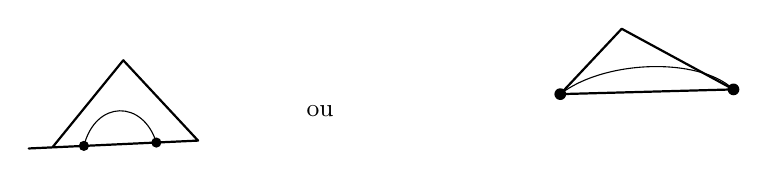
\begin{tikzpicture}[x=1mm,y=1mm,line cap=round,line join=round,font=\small]
\draw[thick] (5,-21.2) -- (26.5,-20.2) -- (17,-10) -- (8,-21.06);
\draw (12,-20.87) .. controls (13.5,-15) and (19.5,-15) .. (21.2,-20.45);
\node[pt, inner sep=1.3pt] at (12,-20.87) {};
\node[pt, inner sep=1.3pt] at (21.2,-20.45) {};
\node[inner sep=1pt] at (42,-16.5) {\small ou};
\draw[thick] (72.5,-14.3) -- (94.5,-13.7) -- (80.3,-6) -- cycle;
\draw (72.5,-14.3) .. controls (78,-10) and (90,-9.5) .. (94.5,-13.7);
\node[pt, inner sep=1.5pt] at (72.5,-14.3) {};
\node[pt, inner sep=1.5pt] at (94.5,-13.7) {};
\end{tikzpicture}
\end{document}
